\section{Le découpage}
%*****************************************************************
\subsection{Pourquoi découper ?}
\frame{
\frametitle{Pourquoi découper ?}

\begin{itemize}
\item<+-> Faire face à la complexité des activités\\
      (``diviser pour régner'')
\item<+->  Aborder le projet en termes d'unités de fabrication\\
      (Toujours se souvenir de l'objectif final)
      
\item<+->  Diminuer les risques de dérives\\
      (Cloisonnement des activités)

\item<+->  Affecter des activités aux acteurs\\
      (Faire correspondre besoins et compétences)
      
\item<+->  Ordonnancer\\
      (Planifier le travail sur un calendrier)
\end{itemize} 
}
%*****************************************************************
\subsection{Principe du découpage}
\frame{
\frametitle{Principes du découpage}
 
\begin{itemize}
\item<+-> \textbf{Objets} du  découpage : des éléments autonomes
 	\begin{itemize}
 	\item<+->  qui produisent un résultat final
 	\item<+->  qui ont une charge mesurable
 	\item<+->  dont on peut identifier leurs contraintes d'antériorité
	\end{itemize}
	\vspace{5mm}
\item<+-> \textbf{Méthodes} courantes de découpage 
	\begin{itemize}
	\item<+-> sur critère temporel : succession d'étapes et de phases
	\item<+-> sur critère  structurel : définition des modules
	\end{itemize}
\end{itemize} 
}
%*****************************************************************
\begin{comment}
\subsection{Difficultés du découpage}
\frame{
\frametitle{Difficultés du découpage}

Travail très général. Quelques unes des difficultés :\\
\begin{itemize}
\item Identifier précisemment les tâches\\ 
 
\item Recenser les lots à fabriquer\\
 
\item Ne pas oublier de tâches\\
 
\end{itemize}
}
\end{comment}
%*****************************************************************
\subsection{Les méthodes}
\frame{
\frametitle{Choisir une méthode de découpage}

\begin{itemize}
\item<+->  Méthode générale, comme
\begin{itemize}
\item PBS (\emph{Product Breakdown Structure})
\item WBS (\emph{Work Breakdown Structure})
\item OBS (\emph{Organisation Breakdown Structure})
\end{itemize}
\vspace{5mm}

\item<+-> Méthode plus spécifique, caution pour une communauté :\\
      ex : Norme de conduite de projet AFNOR Z67-101
\vspace{5mm}

\item<+-> Méthodes de conception spécifique métier :\\
      Exemple pour les développements informatiques :
	\begin{itemize}
		\item Merise
		\item SADT
		\item UML 
	\end{itemize}
\end{itemize}
}

%*****************************************************************
\frame{
\frametitle{Méthodes PBS/WBS/OBS}

\begin{itemize}
\vspace{5mm}
\item 
PBS : vue hiérarchique des composants, parties, sous-parties,
nécessaires à la construction du produit.

\vspace{5mm}
\item
WBS : division hiérarchique du travail global à réaliser
en \emph{work packages} (ou \emph{lots de travail}), qui peuvent être
estimés, planifiés, et affectés à un responsable (personne ou service).

\vspace{5mm}
\item
OBS : hierarchie de l'organisation qui mène le projet, qui permet.
de mettre en relation PBS avec WBS pour identifier
les responsabilités vis-à-vis des work-packages.

\end{itemize}
}


%*****************************************************************
\frame{
\frametitle{PBS-WBS-OBS}
\begin{center}
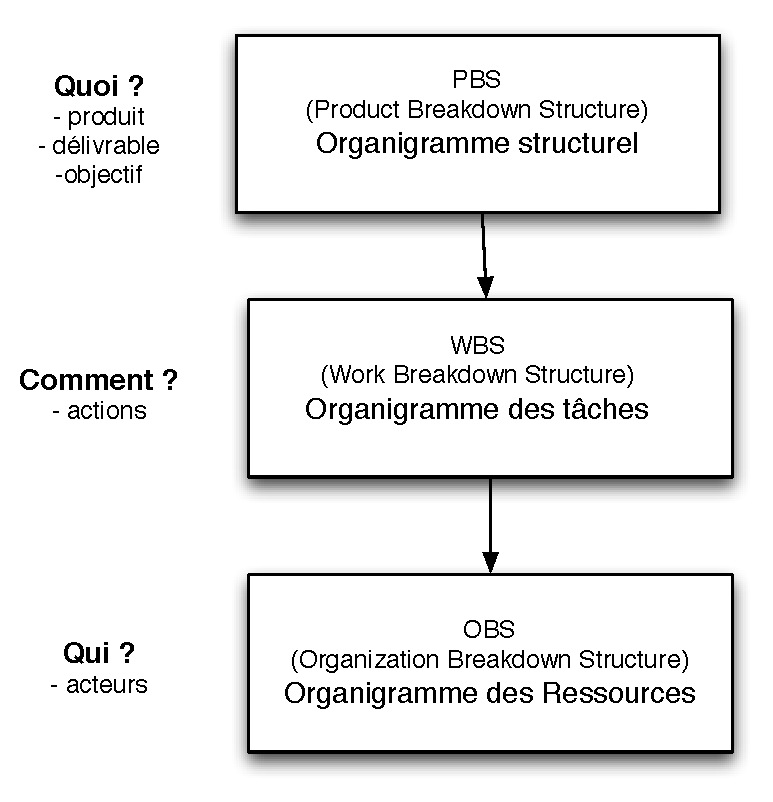
\includegraphics[height=.8\textheight]{pbs-wbs-obs.pdf} 
\end{center}
\vfill  
}
%*****************************************************************
\frame{
\frametitle{Exemple PBS (Product)}
\vspace{1cm}
Découpage PBS (formalisme graphique)
%--------------
%exportée à 70%
%--------------
\[ \input decoupe_PBS.pdftex_t \]
\vfill  
}

%*****************************************************************
\frame{
\frametitle{Exemple WBS (Work)}
\vspace{1cm}

Découpage WBS (formalisme graphique)
%--------------
%exportée à 70%
%--------------
\[ \input decoupe_WBS.pdftex_t \]

\vfill  
}
%*****************************************************************
\frame{
\frametitle{Relation OBS/WBS}
\vspace{1cm}

Relation  OBS/WBS $\Rightarrow$ Responsabilités vis-à-vis du produit

\[ \input decoupe_OWBS.pdftex_t \]

Aussi désignée par \emph{Responsibility Assignment Matrix} (RAM)
}
%*****************************************************************
\frame{
\frametitle{Exemple WBS : institut de formation}

Pour la gestion d'un institut on identifié 4 domaines:
\begin{itemize}
\item gestion des candidatures 
\item gestion des demandes de stages
\item gestion des stages
\item suivi budgétaire
\end{itemize}
Pour chaque domaine, on décrit la succession des 
travaux à mener. Par exemple:
}

\frame{
\frametitle{Exemple WBS : institut de formation}
\begin{center}
\fbox{\begin{minipage}[t]{8cm}
\begin{tabbing}
xxxx\=xxx\=xxx\=xxx\=xxx\= \kill
Application 1 : \textbf{Gestion des candidatures}\\
\> 1. Etude préalable\\
\>\> 11. Lancement de la phase  \\
\>\> 12. Recueil de l'existant\\
\>\> 13. Conception\\
\>\> 14. Appréciation \\
\>\> 15. Validation de la phase\\
\>2. Etude détaillée\\
\>\> 21. Conception fonctionnelle générale\\
\>\> 22. Conception fonctionnelle détaillée\\
\>\> 23. Conception technique et validation\\
\>3. Réalisation\\
\>\> 31. Etude technique\\
\>\> 32. Production du logiciel
\end{tabbing}
\end{minipage}}\end{center}
 
}
%*****************************************************************
\frame{\frametitle{exemple : institut de formation (2)}

on raffine: 
\begin{center}
\fbox{\begin{minipage}[t]{8cm}
\begin{tabbing}
xxxx\=xxx\=xxx\=xxx\=xxx\= \kill
\> 1. Etude préalable\\
\>\> 14. Appréciation\\
\>\>\> 141. Etude des scénarios de développement\\
\>\>\> 142. Elaboration du bilan\\
\>\>\> 143. Rédaction du dossier de choix\\
\>\>\> 143. Réunion du comité directeur\\
\end{tabbing}
\end{minipage}}\end{center}

\begin{center}
\fbox{\begin{minipage}[t]{8cm}
\begin{tabbing}
xxxx\=xxx\=xxx\=xxx\=xxx\= \kill
\> 142. Elaboration du bilan\\
\>\> 1421. Recueil des éléments de coûts\\
\>\> 1422. Recherche des éléments de gains attendus\\
\>\> 1423. construction des bilans par scénario\\
\end{tabbing}
\end{minipage}}\end{center}
}


%*****************************************************************
\frame{
\frametitle{Exemple: projet minier}


Le projet est de \textbf{déterminer la faisabilité d'une exploitation minière}.

Sont identifiées:

\begin{itemize}
\item la liste de tâches
\item les ressources 
\end{itemize}

Déterminer le PBS, le WBS puis l'OBS pour ce projet.

}


%*****************************************************************
\frame{
\frametitle{Synthèse WBS/PBS/OBS}

\begin{itemize}
\item La méthode est générale, et peut s'appliquer à tout projet.\\

\item Certaines spécifités du métiers
      ne sont pas prises en compte (trop générale).\\

\item La structure hiérarchique arborescente favorise un découpage
      récursif des éléments.\\
      
\item Dans la pratique, on utilise des patrons (templates) définis pour un type de projet donné.\\
Exemple : l'armée U.S. demande à ses sous-traitants de se conformer 
au WBS normalisé US MIL-STD-881.
\end{itemize}

}
%*****************************************************************
\subsection{Decoupage en phases}
\frame{
\frametitle{Découpage en phases}
On retrouve généralement les phases suivantes, terminées par une procédure de validation.

\pause

\begin{enumerate}
\item	<2,8> \textbf{\'{E}tude de faisabilité} 
\small{(ou \textbf{préliminaire}, \textbf{préalable}, \textbf{d'opportunité})}

\item	<3,8> \textbf{Lancement}

\item	<4,8> \textbf{Définition des solutions}

\item	<5,8> \textbf{Conception détaillée}

\item	<6,8> \textbf{Réalisation}

\item	<7,8>\textbf{Recette}

\end{enumerate}

%-------------------- frame etude detaillée ---------
 \only<2>{
      \begin{tabular}{|p{\textwidth}|}
      \hline
      -- dététerminer le périmètre (ce qui sera inclus dans les objectifs),\\
      -- sa faisabilité technique (e.g. étude de terrain, recherche de solution existante),\\
      -- les compétences requises, les compétences à acquérir,\\
      -- les risques de faire, les risques de ne pas faire, éventuellement le retour sur investissement attendu.\\
      \hline
      \end{tabular}
}
%-------------------- frame lancement ---------
\only<3>{
      \vspace{3mm}
      \begin{tabular}{|p{\textwidth}|}
      \hline 
      -- on définit l'organisation du projet (chef de projet, comité pilotage, experts, sous-traitants),\\
      -- les moyens de contrôler les résultats,\\
      -- les engagements budgétaires.\\
      \hline
      \end{tabular}
}

%-------------------- frame def. solution ---------
\only<4>{
      \vspace{3mm}
      \begin{tabular}{|p{\textwidth}|}
      \hline 
      -- étude de différentes solutions ou architectures techniques possibles,\\
      -- appel d'offre éventuels auprès de sous-traitants,\\
      -- réalisation d'un prototype,\\
      -- éventuellement, mise sur un marché test.\\
      \hline
      \end{tabular}
}
%-------------------- frame conception detaillee ---------
\only<5>{
      \begin{tabular}{|p{\textwidth}|}
      \hline 
      -- représentation précise de l'objectif à travers les spécifications,\\
	-- contrats de réalisation, cahier des charges fournisseurs.\\
      \hline 
      \end{tabular}
}
%-------------------- frame realisation ---------
\only<6>{
      \vspace{3mm}
      \begin{tabular}{|p{\textwidth}|}
      \hline 
	-- la fabrication même du produit final\\
      -- tests (unitaires, d'intégration, de performance)\\
      \hline 
      \end{tabular}
}
%-------------------- frame recette ---------
\only<7>{
      \vspace{3mm}
      \begin{tabular}{|p{\textwidth}|}
      \hline 
      -- vérification globale avec accompagnement (formation, conduite du changement, ...).\\
      -- réception, qualification, certification, homologation, simulation.\\
      \hline 
      \end{tabular}
}

%-------------------- fin des frames ---------
\pause
}

%*****************************************************************
\frame{
\frametitle{Norme AFNOR}

Norme Z67-101 "recommandations pour la conduite de projets informatiques"
s'inspire de la méthode Merise et normalise le découpage
du processus de développement.

\begin{center}
\begin{small}
\begin{tabular}{|ll|}
\hline
1. \'{E}tude préalable		& $\left\{\begin{tabular}{ll}
				Exploration \\
				Conception d'ensemble\\
				Appréciation solution
			  \end{tabular}\right.$\\
\hline
2. Conception détaillée	& $\left\{\begin{tabular}{ll}
				Conception du S.I.\\
				Spécifications fonctionnelles\\
				Etude organique générale
			  \end{tabular}\right.$\\
\hline			  
3. Réalisation	& $\left\{\begin{tabular}{ll}
				Etude organique détaillée\\
				Programmation et tests\\
				Validation technique
			  \end{tabular}\right.$\\
 \hline
4. Mise en oeuvre	& $\left\{\begin{tabular}{ll}
				Réception provisoire\\
				Exploitation sous contrôle
			  \end{tabular}\right.$\\
\hline			  
5. \'{E}valuation	& $\left\{\begin{tabular}{ll}
				 Evaluation du système info.\\
				 Evaluation du S.I.
			  \end{tabular}\right.$\\\hline	  
\end{tabular}
\end{small}
\end{center}
}
